%!TEX root = ../thesis.tex

\chapter{Precision, Hardware, and Implementation Results}
\label{chap:variation-results}

\section{Result matrix overview}
\label{sec:ch5-matrix-overview}

Chapter~4 established the validation limits within which variation could be
interpreted. This chapter changes the precision, effective build semantics,
solver, device, resolution, observation time, thread count, or CFL number in
the matched groups defined in Chapter~3. Each observation remains conditional
on its stated case, baseline, metric, and configuration.

\section{Deterministic output sensitivity}
\label{sec:ch5-deterministic-sensitivity}

\subsection{Euler--MHD cross-system sensitivity}
\label{sec:ch5-cross-system}

Figure~\ref{fig:ch5-cross-system} provides the compact continuity test across
Sod, Liska--Wendroff Configuration~3, Brio--Wu, and Orszag--Tang; all 16
configured runs completed. For the four O2-default fp32--fp64 pairs, density
mean-relative $L_1$ differences ranged from $1.377\times10^{-7}$ to
$3.762\times10^{-7}$; retained $L_\infty$ values ranged from
$3.837\times10^{-7}$ to $5.254\times10^{-6}$.

Sod and LW3 used Euler HLLC, whereas Brio--Wu and Orszag--Tang used ideal-MHD
HLL with different grids and final times. The figure shows measurable
fp32--fp64 differences; it does not rank systems or solvers, or repeat
Report~1 validation.

% Source PDF SHA-256:
% beb1b8d134470983c1987cffa795456e2e354df75239571e8d47b243f7003e8d
\begin{figure}[htbp]
\centering
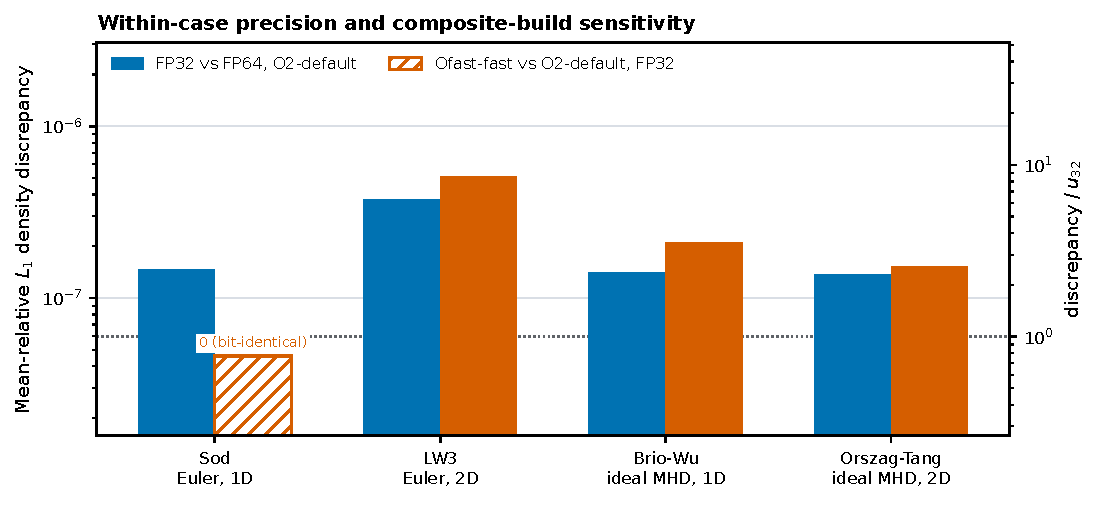
\includegraphics[width=\textwidth]{Figs/report2/ch5_cross_system_sensitivity}
\caption[Euler--MHD density sensitivity]{\textbf{Euler--MHD density
sensitivity.} Matched density mean-relative $L_1$ differences for fp32 versus
fp64 and the composite Ofast-fast versus O2-default build pair. Each bar uses
its declared within-row baseline. Sod and Brio--Wu used $N=200$ and 800;
LW3 and OT used $200^2$ and $128^2$. Euler uses HLLC and MHD uses HLL, so the
panels do not compare cross-system accuracy or rank solvers.}
\label{fig:ch5-cross-system}
\end{figure}

\subsection{Deterministic fp32--fp64 sensitivity}
\label{sec:ch5-deterministic-precision}

Within the two MHD rows in Figure~\ref{fig:ch5-cross-system}, the
Brio--Wu and Orszag--Tang density mean-relative $L_1$ differences were
$1.401\times10^{-7}$ and $1.377\times10^{-7}$, with $L_\infty$ differences of
$1.075\times10^{-6}$ and $3.565\times10^{-6}$, respectively. The separate KH
comparison at $256^2$, $t=1.0$, and CFL 0.4 gave density $L_\infty$
differences of $1.786\times10^{-6}$ for HLL and $3.230\times10^{-6}$ for HLLD.
Each value compares fp32 with its same-solver fp64 numerical baseline.

These values quantify arithmetic sensitivity, not exact-state or
discretisation error, and do not establish fp32 adequacy beyond these rows.
Brio--Wu has matched deterministic/MCA scope; the smaller, earlier
Orszag--Tang MCA scope remains separate in
Appendix~\ref{sec:appendix-ch5-mca-status}.

\subsection{Effective build-semantics sensitivity}
\label{sec:ch5-build-sensitivity}

The build pair in Figure~\ref{fig:ch5-cross-system} compared effective
O2-default and Ofast-fast semantics. In fp64, the
mean-relative density response lay between $4.24\times10^{-17}$ and
$4.21\times10^{-16}$. In fp32 it ranged from exactly zero for Sod to
$5.124\times10^{-7}$ for LW3. Because this pair changed several recorded
semantics, it does not identify a cause.

At $N=800$, $t=0.1$, CFL 0.4 and one thread, a clean MSVC~19.51 Brio--Wu
rebuild varied one recorded axis per pair. All four /Ox--/O2 density
discrepancies were zero. For
/fp:fast versus compiler-default math, $L_\infty$ was
$1.887\times10^{-15}$ and $1.311\times10^{-6}$ for HLL, and
$4.413\times10^{-15}$ and $1.729\times10^{-6}$ for HLLD, in fp64 and fp32.
Changing the Riemann branch from $\leq$ to $<$ gave zero for both HLL groups,
but $3.886\times10^{-15}$ and $2.608\times10^{-6}$ for HLLD. These density
responses are not compiler-wide, performance, or accuracy claims.

\section{Solver and device performance}
\label{sec:ch5-performance}

\subsection{HLL and HLLD timing comparison}
\label{sec:ch5-solver-timing}

Changing HLL to HLLD changes the numerical method rather than reproducing the
same implementation. Figure~\ref{fig:ch5-kh-timing} therefore compares timing
only within a fixed $256^2$ KH configuration at $t=1.0$, CFL 0.4, and one
OpenMP thread. The fp64 medians were 34.484~s for HLL and 39.542~s for HLLD;
the fp32 medians were 29.196~s and 34.254~s. All groups took 1148 steps. FP32 was
$1.181\times$ faster for HLL and $1.154\times$ faster for HLLD, while the
HLLD/HLL median cost ratios were 1.147 in fp64 and 1.173 in fp32.

After one excluded warm-up, all 20 measured outputs were bit-identical within
their group. The timings establish neither an accuracy--cost trade-off nor a
portable solver ranking; Chapter~4 also used different solver-specific CFL
numbers.

% Source PDF SHA-256:
% 12e0140c6302bbbcd98ce8845c2a46a483c6632dcadcf598b7f2cf09fea85358
\begin{figure}[htbp]
\centering
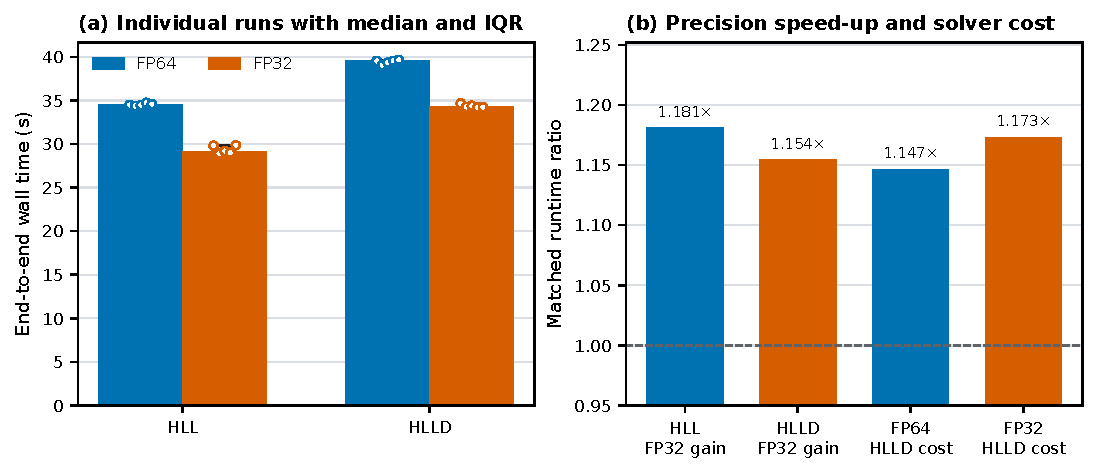
\includegraphics[width=\textwidth]{Figs/report2/ch5_kh_timing}
\caption[KH solver and precision timing]{\textbf{KH solver and precision
timing.} Median subprocess wall time, interquartile range and five observations
after one excluded warm-up per HLL/HLLD and fp64/fp32 group. The runs used
$256^2$, $t=1.0$, CFL 0.4, and one OpenMP thread on one workstation. All 20
outputs had zero within-group ULP drift; this is not an accuracy--cost or
cross-machine result.}
\label{fig:ch5-kh-timing}
\end{figure}

\subsection{Matched CPU/GPU agreement and performance}
\label{sec:ch5-hardware}

Table~\ref{tab:ch4-cpu-gpu} established zero ULP and zero absolute drift for
the covered CPU/GPU saved-state pairs. The five-repeat results in
Figure~\ref{fig:ch5-hardware} preserve that equality. For Brio--Wu, the CPU/GPU
median per-repeat wall-time ratios were 0.510 in fp64 and 0.488 in fp32, so GPU
execution took longer. For the $256^2$ Orszag--Tang workload, the corresponding
ratios were 6.174 and 5.925, so GPU execution took less time on the same
workstation.

The timing contrast changed sign between workloads. The measurements did not
separate transfer, launch, I/O, and compute time, so they do not identify its
cause. The subprocess timer included required output. Coverage is limited to
HLL Brio--Wu and Orszag--Tang in two precisions, excluding HLLD, KH, GPU MCA,
other devices, and general hardware independence. The raw points also show one
Brio--Wu fp64 GPU observation of 2.695~s, whereas the other four were
0.305--0.317~s. No device warm-up was excluded, so the median is retained but
the outlier is not interpreted.

% Source PDF SHA-256:
% 643820272d5a8cedc0ca6235a280b66d751fc4764fe65b80fe6c13ad470aba7c
\begin{figure}[htbp]
\centering
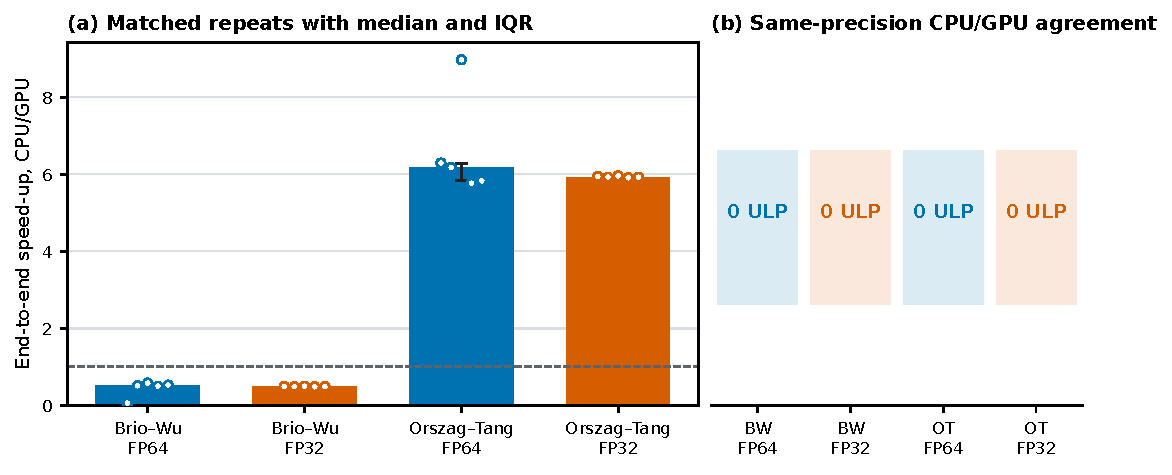
\includegraphics[width=\textwidth]{Figs/report2/ch5_hardware_reproducibility}
\caption[Repeated CPU/GPU agreement and timing]{\textbf{Repeated CPU/GPU
agreement and timing.} Median, interquartile range and five matched
per-repeat CPU/GPU wall-time ratios for HLL Brio--Wu ($800\times1$) and
Orszag--Tang ($256^2$) in fp64 and fp32 on the tested workstation.
Same-precision comparisons had zero maximum ULP. This is not a general
GPU-performance claim.}
\label{fig:ch5-hardware}
\end{figure}

\section{Scale, time, and stochastic sensitivity}
\label{sec:ch5-scale-time-stochastic}

\subsection{Resolution dependence of discrepancies}
\label{sec:ch5-resolution-precision}

The three-grid matrix contained eight complete self-refinement groups and 12
complete same-grid fp32--fp64 cells. Figure~\ref{fig:ch5-precision-refinement}
shows the mean-$L_1$ precision discrepancy $D_N$ rather than the observed-order
statistic plotted in Chapter~4. Within each matched case and solver,
$D_N/E^{64}_{256,512}$ ranged from $4.95\times10^{-6}$ to
$2.76\times10^{-2}$. Thus every covered mean-$L_1$ precision discrepancy was
below 3\% of the matched fp64 finest adjacent-grid difference.

The maximum norm was more sensitive to local extrema. For the corrected
Orszag--Tang HLLD pair at $512^2$, $t=0.5$, and CFL 0.2, density mean-$L_1$ was
$5.554\times10^{-5}$ while $L_\infty$ was $5.031\times10^{-2}$. The ratio in
Figure~\ref{fig:ch5-precision-refinement} is therefore a refinement-scale
context for one norm, not exact error, an fp32-adequacy test, asymptotic
convergence, or a cross-solver ranking.

% Source PDF SHA-256:
% 51ad93f4fd9ebba37fe868da105e360a29785b82dd7faf57af2a6d001914c68c
\begin{figure}[htbp]
\centering
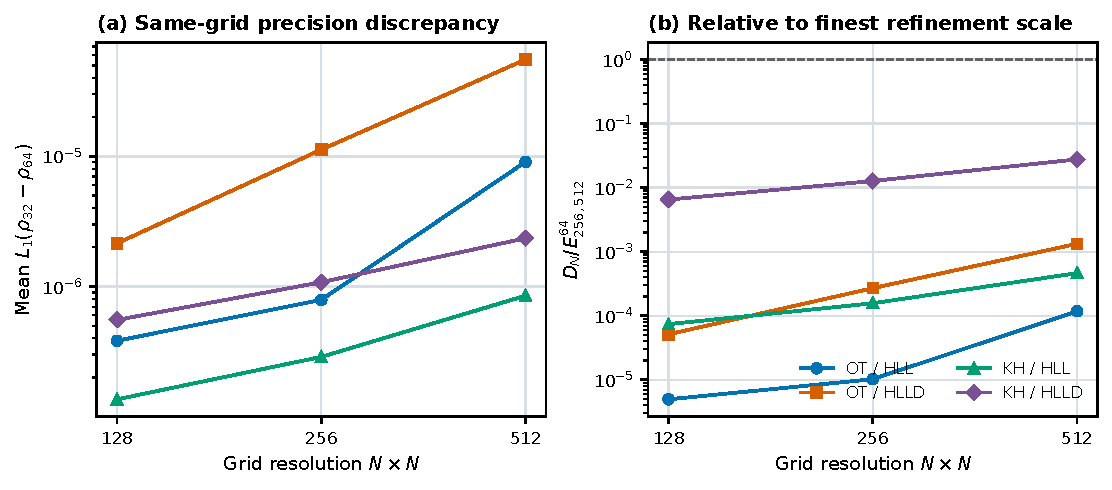
\includegraphics[width=\textwidth]{Figs/report2/ch5_precision_refinement_context}
\caption[Precision discrepancy relative to refinement scale]{\textbf{Precision
discrepancy relative to refinement scale.} (a) Same-grid density mean-$L_1$
for fp32 versus fp64 across all 12 matched OT/KH, HLL/HLLD and resolution cells.
(b) The same discrepancy divided by the matched fp64 $256^2$--$512^2$
adjacent-grid mean-$L_1$ difference. The denominator is a numerical refinement
scale, not an exact error. OT used $t=0.5$ and KH $t=1.0$; HLL used CFL 0.4
and HLLD CFL 0.2.}
\label{fig:ch5-precision-refinement}
\end{figure}

\subsection{Growth of discrepancies with time}
\label{sec:ch5-temporal}

The temporal test used 15 aligned Brio--Wu pairs and 25 aligned Orszag--Tang
pairs, with fixed log-linear windows of $[0.01,0.1]$ and $[0.1,0.5]$.
Figure~\ref{fig:ch5-temporal} shows a Brio--Wu mean-$L_1$ slope of 30.6153 with
$R^2=0.963$; its $L_\infty$ fit gave $R^2=0.852$. Orszag--Tang instead gave
slopes of 0.02934 and $-0.04223$, with $R^2=0.0073$ and 0.0006, so the declared
log-linear model explained almost none of its fixed-window variation.

The case time coordinates do not share a demonstrated characteristic-time
normalisation. Their raw slopes are therefore reported within case, not treated
as transferable physical rates. The planned faster Orszag--Tang separation was
not supported because no log-linear Orszag--Tang trend was detected in the
declared window; these fits are not maximal Lyapunov exponents.

% Source PDF SHA-256:
% 901f855f9ea612da2886c6632c400f2f56403bc67ee7fd8ddfb847fb6831d2bf
\begin{figure}[htbp]
\centering

\includegraphics[width=\textwidth]{Figs/report2/ch5_temporal_discrepancy}
\caption[Fixed-window fp32--fp64 temporal discrepancy]{\textbf{Fixed-window
fp32--fp64 temporal discrepancy.} Density mean $L_1$ and $L_\infty$ from 15
aligned Brio--Wu pairs and 25 aligned Orszag--Tang pairs. Fits use the fixed
$[0.01,0.1]$ and $[0.1,0.5]$ windows with HLL at $N=800$ and $128^2$.
The raw slopes are case-specific;
near-zero Orszag--Tang $R^2$ shows that its declared log-linear model did not
describe the fixed-window variation.}
\label{fig:ch5-temporal}
\end{figure}

\subsection{Monte Carlo arithmetic}
\label{sec:ch5-mca}

The MCA runs used Verificarlo compiler instrumentation
\citep{denisEtAl2016verificarlo}. Table~\ref{tab:ch5-mca-primary} retains only
the same-scope Brio--Wu packets at $N=800$ and $t=0.1$. The p24 maximum spreads
were 2.12 and 2.46 times the deterministic fp32--fp64 $L_\infty$ differences
for HLL and HLLD. This is an order-of-magnitude context, not an equality of
statistics or an identification of virtual p24 with IEEE fp32.

The Orszag--Tang MCA rows used $64^2$, $t=0.05$ rather than the deterministic
$256^2$, $t=0.5$ scope and are not combined. Reduced KH validation and the
unavailable full KH scope are recorded in
Table~\ref{tab:appendix-ch5-mca-status}; neither supports a full-scale KH MCA
magnitude.

\begin{table}[htbp]
\centering
\small
\begin{tabularx}{\textwidth}{@{}lrrrrX@{}}
\toprule
Solver & Deterministic $L_\infty$ & p53 spread & p24 spread & p24/$L_\infty$ & Scope \\
\midrule
HLL  & $1.075\times10^{-6}$ & $5.117\times10^{-15}$ & $2.275\times10^{-6}$ & 2.12 & $N=800$, $t=0.1$, 30 samples \\
HLLD & $1.629\times10^{-6}$ & $8.442\times10^{-15}$ & $4.007\times10^{-6}$ & 2.46 & $N=800$, $t=0.1$, 30 samples \\
\bottomrule
\end{tabularx}
\caption[Matched Brio--Wu deterministic and MCA scales]{\textbf{Matched
Brio--Wu deterministic and MCA scales.} Deterministic $L_\infty$ is the
fp32--fp64 density difference; MCA spread is the maximum cellwise sample
standard deviation. Their ratio is descriptive because the statistics are not
equivalent. Virtual p24 and p53 are not IEEE fp32 and fp64.}
\label{tab:ch5-mca-primary}
\end{table}


\section{Robustness checks}
\label{sec:ch5-robustness}

\subsection{Thread-count and CFL sensitivity}
\label{sec:ch5-thread-cfl}

For the covered Orszag--Tang and KH configurations, runs with 1, 2, 4, and 8
OpenMP threads all matched the one-thread saved state with zero maximum ULP and
zero absolute drift. This establishes thread-count reproducibility for those
local rows. Because elapsed-time scaling was not the question and no MPI path
was exercised, it says neither that OpenMP scales efficiently nor that MPI
reduction ordering is immaterial.

All KH runs at CFL 0.2, 0.4, 0.6, and 0.8 completed with finite, positive
states. For HLL, the fp32--fp64 density $L_\infty$ values were
$4.678\times10^{-6}$, $1.786\times10^{-6}$, $2.133\times10^{-6}$, and
$8.910\times10^{-7}$ in increasing CFL order. The HLLD values were
$7.204\times10^{-6}$, $3.230\times10^{-6}$, $4.057\times10^{-6}$, and
$3.157\times10^{-6}$. Both responses were non-monotonic, so reducing CFL did
not consistently reduce precision separation. This is a CFL-sensitivity result
rather than formal temporal convergence or a general solver ranking.

\section{Bounded result summary}
\label{sec:ch5-bounded-summary}

Within the covered rows, zero within-group repeat, CPU/GPU, and thread differences distinguish
deterministic reproduction from observed non-zero precision and build
discrepancies or CFL-dependent separation, without defining a common noise
threshold. All 12 mean-$L_1$
precision discrepancies remained below 3\% of their matched fp64 finest
refinement scale; hardware timing differed by workload; and no log-linear
Orszag--Tang discrepancy growth was detected in the declared window. Solver
timing and MCA remain separately scoped and do not define a cross-axis leaderboard.
